\documentclass{article}
\usepackage{graphicx} % Required for inserting images
\usepackage{subcaption}
\usepackage{tikz}
\usepackage{amsmath}
\usepackage{amsfonts}
\usetikzlibrary{positioning,arrows.meta,calc}
\usepackage[galician]{babel}
\usetikzlibrary{matrix, positioning}
\usepackage{caption}
%\usepackage{hyperref}

\title{A beleza da convolución}
\author{Víctor Xesús Barreiro Domínguez \\
\textit{victorxesus.barreiro.dominguez@gmail.com}}
\date{Outubro 2023}

\begin{document}

\maketitle

\tableofcontents

\section{Introdución}

Neste documento quero presentar a conexión entre a idea de convolución empregada en análise funcional e teoría de sinais coa redes convolucionais. Do mesmo xeito, explicaremos como sería posible implemntar unha rede convolucional a través dun perceptrón. Deste xeito, entenderemos porque as redes non son formalmente máis expresivas que un perceptrón multicapa pero na práctica si son máis fáciles de adestrar e moito máis eficientes. 

\section{Imaxe coma función.}

Este enfoque é o máis habitual en visión por computador a hora de aplicar numerosas técnicas xa que nos permite aplicar ferramentas matemáticas dunha forma moi intuitiva, como veremos. 

Unha cuestión a comentar é que na meirande parte dos casos falaremos de funcións continuas xa que para moitos lectores teñan unha maior intuición nestes contextos, todos terán unha intuición sobre unha educación diferencial pero probablemente moitos non teñan escoitado o termo ecuación en diferencias. As implantacións que posteriormente traballaran coa natureza discreta de forma relativamente transparente. 

Deste xeito podemos definir unha imaxe en branco e negro como unha función $f: R^{2} \longrightarrow R$, onde temos que:

\begin{equation}
    f(x, y) \in [0,1] / \; x \in [0,anchura] \wedge y \in [0,altura].
\end{equation}

Probablemente ante esta formalización calquera con tendencia ao rigor chamaralle a atención a forma de definila sobre un dominio \textit{continuo} cando unha imaxe dixital é claramente discreta. Neste sentido cabe destacar que definila deste xeito fainos mais fácil abordar outras cuestións e resulta algo xustificable.

\begin{figure}
    \begin{subfigure}{0.5\textwidth}
    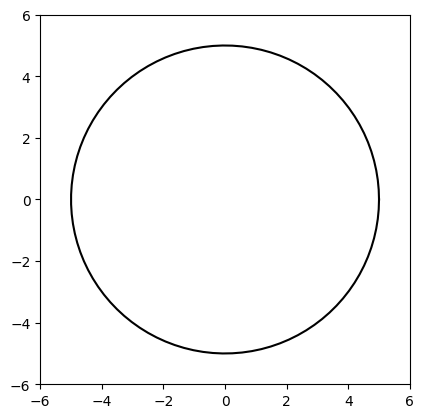
\includegraphics[width=\linewidth]{2D_circle.png}
    \caption{Imaxe.}
    \label{fig:enter-label}
    \end{subfigure}
    \begin{subfigure}{0.5\textwidth}
    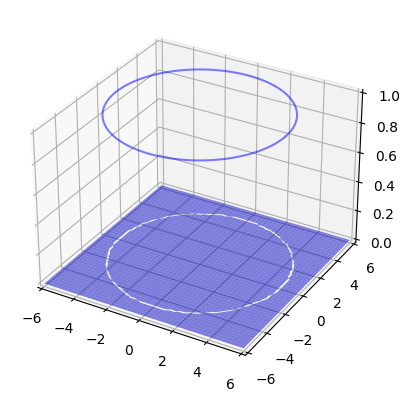
\includegraphics[width=\linewidth]{3D.png}
    \caption{Función.}
    \end{subfigure}
\end{figure}

Por unha banda, se desexasemos ser rigorosos poderíamos facer unha interpolación entre os valores que temos dos pixeles da imaxe para obter unha función nese dominio continuo, porén, non é o habitual xa que moitas das técnicas que veremos disporán de implementacións discretas para aplicar as imaxes reais. Por outra banda, é mais sinxelo amosalo con estes dominios onde físicos, matemáticas e enxeñeiros poden atoparse cómodos lendo. 

Respecto do co-dominio, temos imaxes con valores nese intervalo [0,1] onde a precisión dependerá do nivel de precisión que sexa quen de captar o nosos sensor e a representación máquina. A idea sería equivalente para imaxes nun dominio de enteiros de [0, 255].

\subsection{Dimensións no dominio.}
Neste caso podemos engadir unha dimensión extra ao noso dominio que nos permita ver distintas bandas como as dunha imaxe convencional RGB. 

\begin{equation}
    f(x, y, b) \; \text{onde} \; b \in {bandas}.
\end{equation}

Aínda que se podería pensar que non ten excesivo sentido falar aquí dun continuo, de feito non o estamos indicando, é importante salientar que si o podería ter. Nun contexto, teórico en realidade esta nova dimensión $b$ o que nos está permitindo é desprazarnos no dominio de frecuencias do sinal que estamos procesando a diferencia de $x$ e $y$ que nos permiten movernos no dominio do espazo captado nesta proxección. 

Outro importante enfoque nesta liña de engadir dimensións a nosa función imaxe é engadir a dimensión temporal, a idea de vídeo. Así temos:

\begin{equation}
    f(x, y, t) \; \text{onde} t \in [t_{0}, t_{f}].
\end{equation}

Nun vídeo gravado, $t$ está composto por todos os fotogramas e onde a resolución sería o \textit{frame rate}. Do mesmo xeito, na práctica no semella aportar moito falar dun dominio continuo nesta dimensión do dominio da nosa función, xa que os sistemas electrónicos teñen unha latencia capturando as imaxes. Por contra, volvemos resultar moi útil por familiaridade. 

\section{Convolución.}

Na análise funcional, a convolución é unha operación usada para combinar dúas funcións e producir unha terceira función que representa a forma en que unha función ``inflúe'' na outra. A convolución de dúas funcións \(f\) e \(g\) defínese como
\[
(f * g)(t) = \int_{-\infty}^{\infty} f(\tau) \cdot g(t - \tau) \, d\tau
\]
onde \(t\) é a variable independente e \(\tau\) é unha variable de integración. A convolución é esencialmente un produto integral entre \(f(\tau)\) e \(g(t - \tau)\) despois de desprazar e reflectir \(g\) e despois ``deslizar'' ao longo de \(t\). Esta operación pódese ver como unha forma de medir a ``interación'' entre \(f\) e \(g\) en diferentes puntos de \(t\).

Nota relevante, é \textbf{conmutativa}, \textbf{asociativa} e \textbf{distributiva}.  Ollo é importante parase a pensar a idea e notar que é ben distinto de multiplicar dúas funcións, xa que é unha confusión habitual ao ler explicacións sobre redes convolucionais. 

%\begin{figure}
 %   \centering
  %  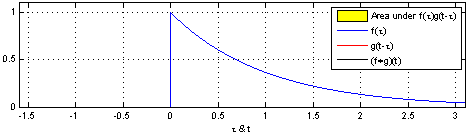
\includegraphics[width=1\linewidth]{image.png}
   % \caption{Exemplo de convolución.}
    %\label{fig:enter-label}
%\end{figure}

\begin{figure}[h]
    \centering
    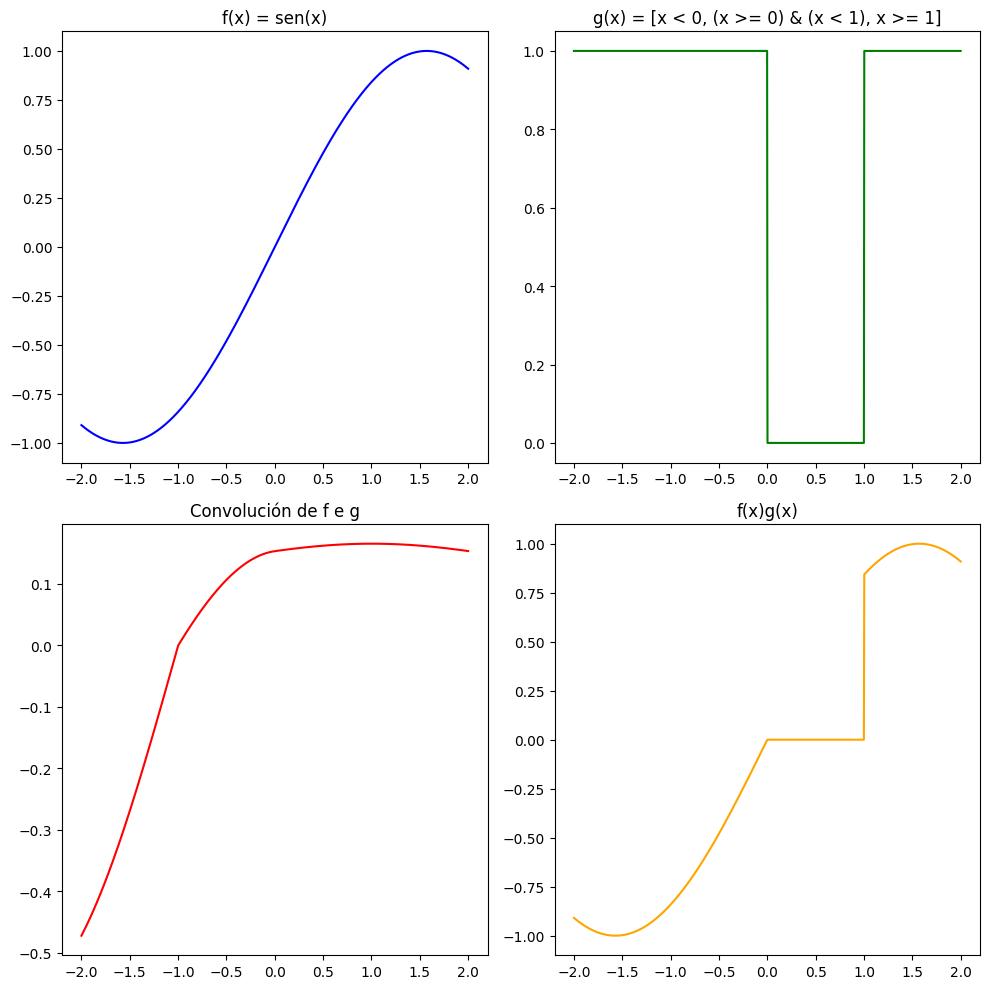
\includegraphics[width=0.9\linewidth]{exampleConvolution.png}
    \caption{Exemplo de convolución.}
    \label{fig:enter-label}
\end{figure}

\section{Perceptrón como convolución numérica. }

\subsection{Neurona e capa dun perceptrón. }
Unha neurona do perceptrón ten a definición \ref{eq_neuron}. Onde a entrada é un vector $X \in \mathbb{R}^n $, con compoñentes $x_i$, é a saída é $y \in \mathbb{R}$.

\begin{equation}
    neurona(X) = f_{act}(\sum_{i=1}^{n} w_i \cdot x_i + b)
    \label{eq_neuron}
\end{equation}

En diante imos ter $neurona: \mathbb{R}^n \rightarrow \mathbb{R}$. Unha nota relevante é que normalmente as entradas tentaremos que estean normalizadas e tentaremos normalizar a saída das capas de xeito que en lugar de $\mathbb{R}$ teremos $[0,1]$. Poñemos agora mítica figuriña chamativa \ref{fig:esq_nerona}. 

\begin{figure}[h]
    \centering
    \tikzset{
  arro/.style={
    ->,
    >=latex
  },
  bloque/.style={
    draw,
    minimum height=1cm,
    minimum width=0.5cm
  }  
}


\begin{tikzpicture}[]
\node[]
  (input)
  {Entrada};
\node[below=of input,label={left:$x_{1} \cdot w_1$}]
  (inputi)
  {};
\node[below=of inputi,label={left:$x_{2} \cdot w_2$}]
  (inputii)
  {};
\coordinate[below=of inputii] (aux);  
\node[below=of aux,label={left:$x_{3} \cdot w_3$}]
  (inputiii)
  {};
\node[below=of inputiii,label={left:$x_{n} \cdot w_n$}]
  (inputiv)
  {};

\node[right=of input]
  (proje)
  {Proxección};
\node[circle,
   draw,minimum size=1cm,orange, %% <-- these are added
   label={above:\textsc{sum}}]
  at (proje|-aux)
  (projei)
  {};

\node[right=of proje]
  (out)
  {Saída};
\node[label={right:$f_{act}(\sum (x_i \cdot w_i ))$}]
  at (out|-aux)
  (outi)
  {};

\foreach \Valor in {i,ii,iii,iv}
{
  \draw[arro] (input\Valor) -- (projei);
}  
\draw[arro] (projei) -- (outi);
\end{tikzpicture}
    \caption{Esquema de neurona}
    \label{fig:esq_nerona}
\end{figure}


Se agora facemos unha capa de neuronas podémola ver como unha función vectorial, $Capa: \mathbb{R}^n \rightarrow \mathbb{R}^k$ onde $k$ é o número de saídas. Así temos a definición \ref{eq_capa}, onde $X$ é o vector con todos os $x_i$.

\begin{equation}
    Capa(X) := (neurona_{j=0}(X), neurona_{j=1}(X), ..., neurona_{j=k}(X))
    \label{eq_capa}
\end{equation}

\subsection{Convolución discreta.}

\textit{\textbf{Nota importante: }Non seguiremos usando os mesmos índicides que nos apartados anteriores. }

Agora imos recuperar a convolución, e ter en conta que a nosa función de partida é discreta, xa que ao dixitalizar calquera sinal estámolo discretizando. Notar que estamos discretizando o dominio, non o co-dominio. 

A integral segue sendo a mesa, pero neste caso podémola computar directamente xa que podemos percorrer todo o dominio sumando o valor que toma a nosa función para cada elemento do dominio.

Así temos, a convolución discreta de dúas sucesións $f[n]$ e $g[n]$ defínese como:

\begin{equation}
    (f * g)[n] = \sum_{k=-\infty}^{\infty} f[k] \cdot g[n - k]
    \label{eq_convdiscreta}
\end{equation}

Onde:
\begin{itemize}
\item $f[n]$ é unha sucesión, a miúdo chamada "sinal de entrada".
\item $g[n]$ é outra sucesión, a miúdo chamada "filtro".
\item $(f * g)[n]$ é a sucesión resultante da convolución.
\end{itemize}

O índice $n$ representa a posición na sucesión resultante. A suma realízase sobre todos os valores posibles de $k$. É importante ter en conta que as dúas funcións (ou sucesións) poden ter dominios distintos. 

Nas convolucións discretas o habitual é falar de sucesións. É importante ter en conta que unha sucesión é unha función con dominio en $\mathbb{N}$.

Isto é importante xa que unha imaxe é un sinal ou función con dominio de dimensión 2 (normalmente) é discreto. 

\subsection{Redes convolucionais: Unha capa convolucional - unha convolución..}


No noso caso o que imos facer é ter como entrada a nosa imaxe (xa vimos que podemos interpretala coma unha función) e calcular a función que vai actuar coma \textbf{filtro}. 

Á nova función que calcularemos para realizar a nosa convolución chamarémoslle \textbf{kernel}. Convén destacar que na implementación non só faremos a suma pesada como vimos na Definición \ref{eq_convdiscreta}, imos engadirlle unha función de activación ao valor de saída. Engadir esta función aportanos máis expresividade a hora de extraer información concatenando capas, pero para a nosa explicación non é relevante máis aló de que cadra mellor todo como se ve na Figura \ref{fig:exp_equivalanciaconvpercp}.

Agora debemos recoller a función $Capa$ que definimos antes na Definición \ref{eq_capa}. Unha forma de implementar a convolución mediante o perceptron sería fixar a 0 todos os pesos $w_i$ que se correspondan con pixeles que non inflúan no cálculo do novo pixel de saída. Os pesos que non tomen o valor 0 compartiran os mesmos valores pero con un desprazamento. Nas figuras non estamos usando \textit{padding} (recheo) polo que diminúe o tamaño do vector de saída respecto do tamaño do vector de entrada (dominio da función entrada e da función saída). Habitualmente usase \textit{padding} 0 e un desprazamento \textit{``stride''} de 1. Podese ver isto na Figura \ref{fig:exp_equivalanciaconvpercp}.


\begin{figure}[h]
    \centering
    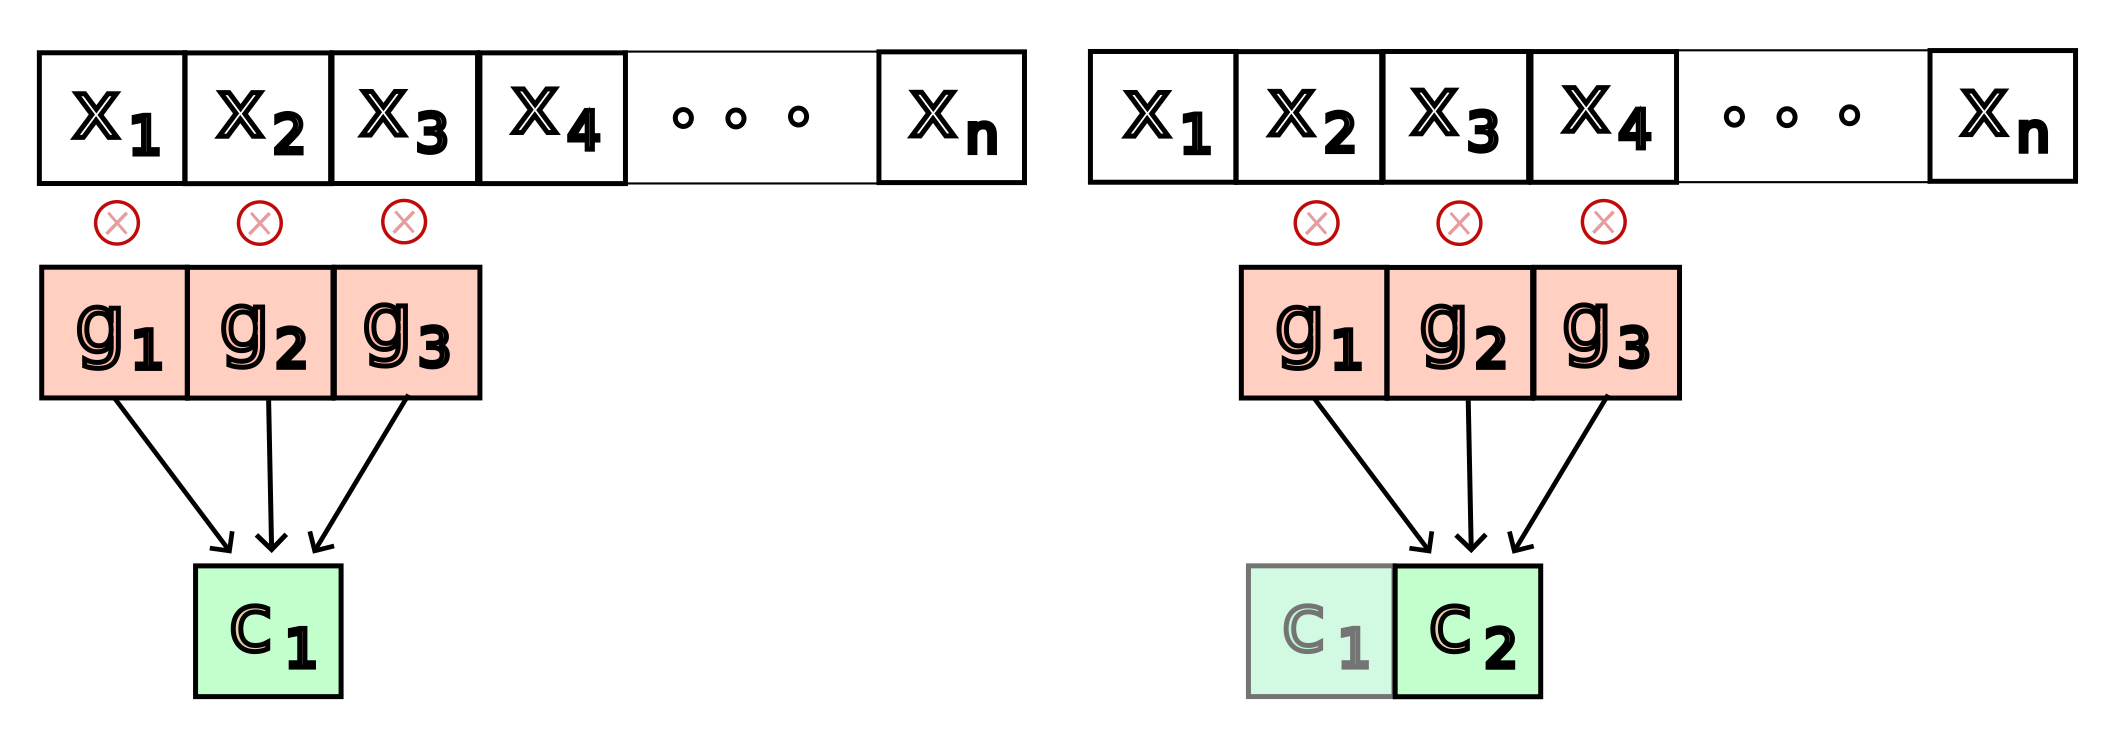
\includegraphics[width=1\linewidth]{CoonvVecDiscreta.png}
    \caption{Convolución disreta sobre un vector.}
    \label{fig:enter-label}
\end{figure}

\begin{figure}
    \centering
    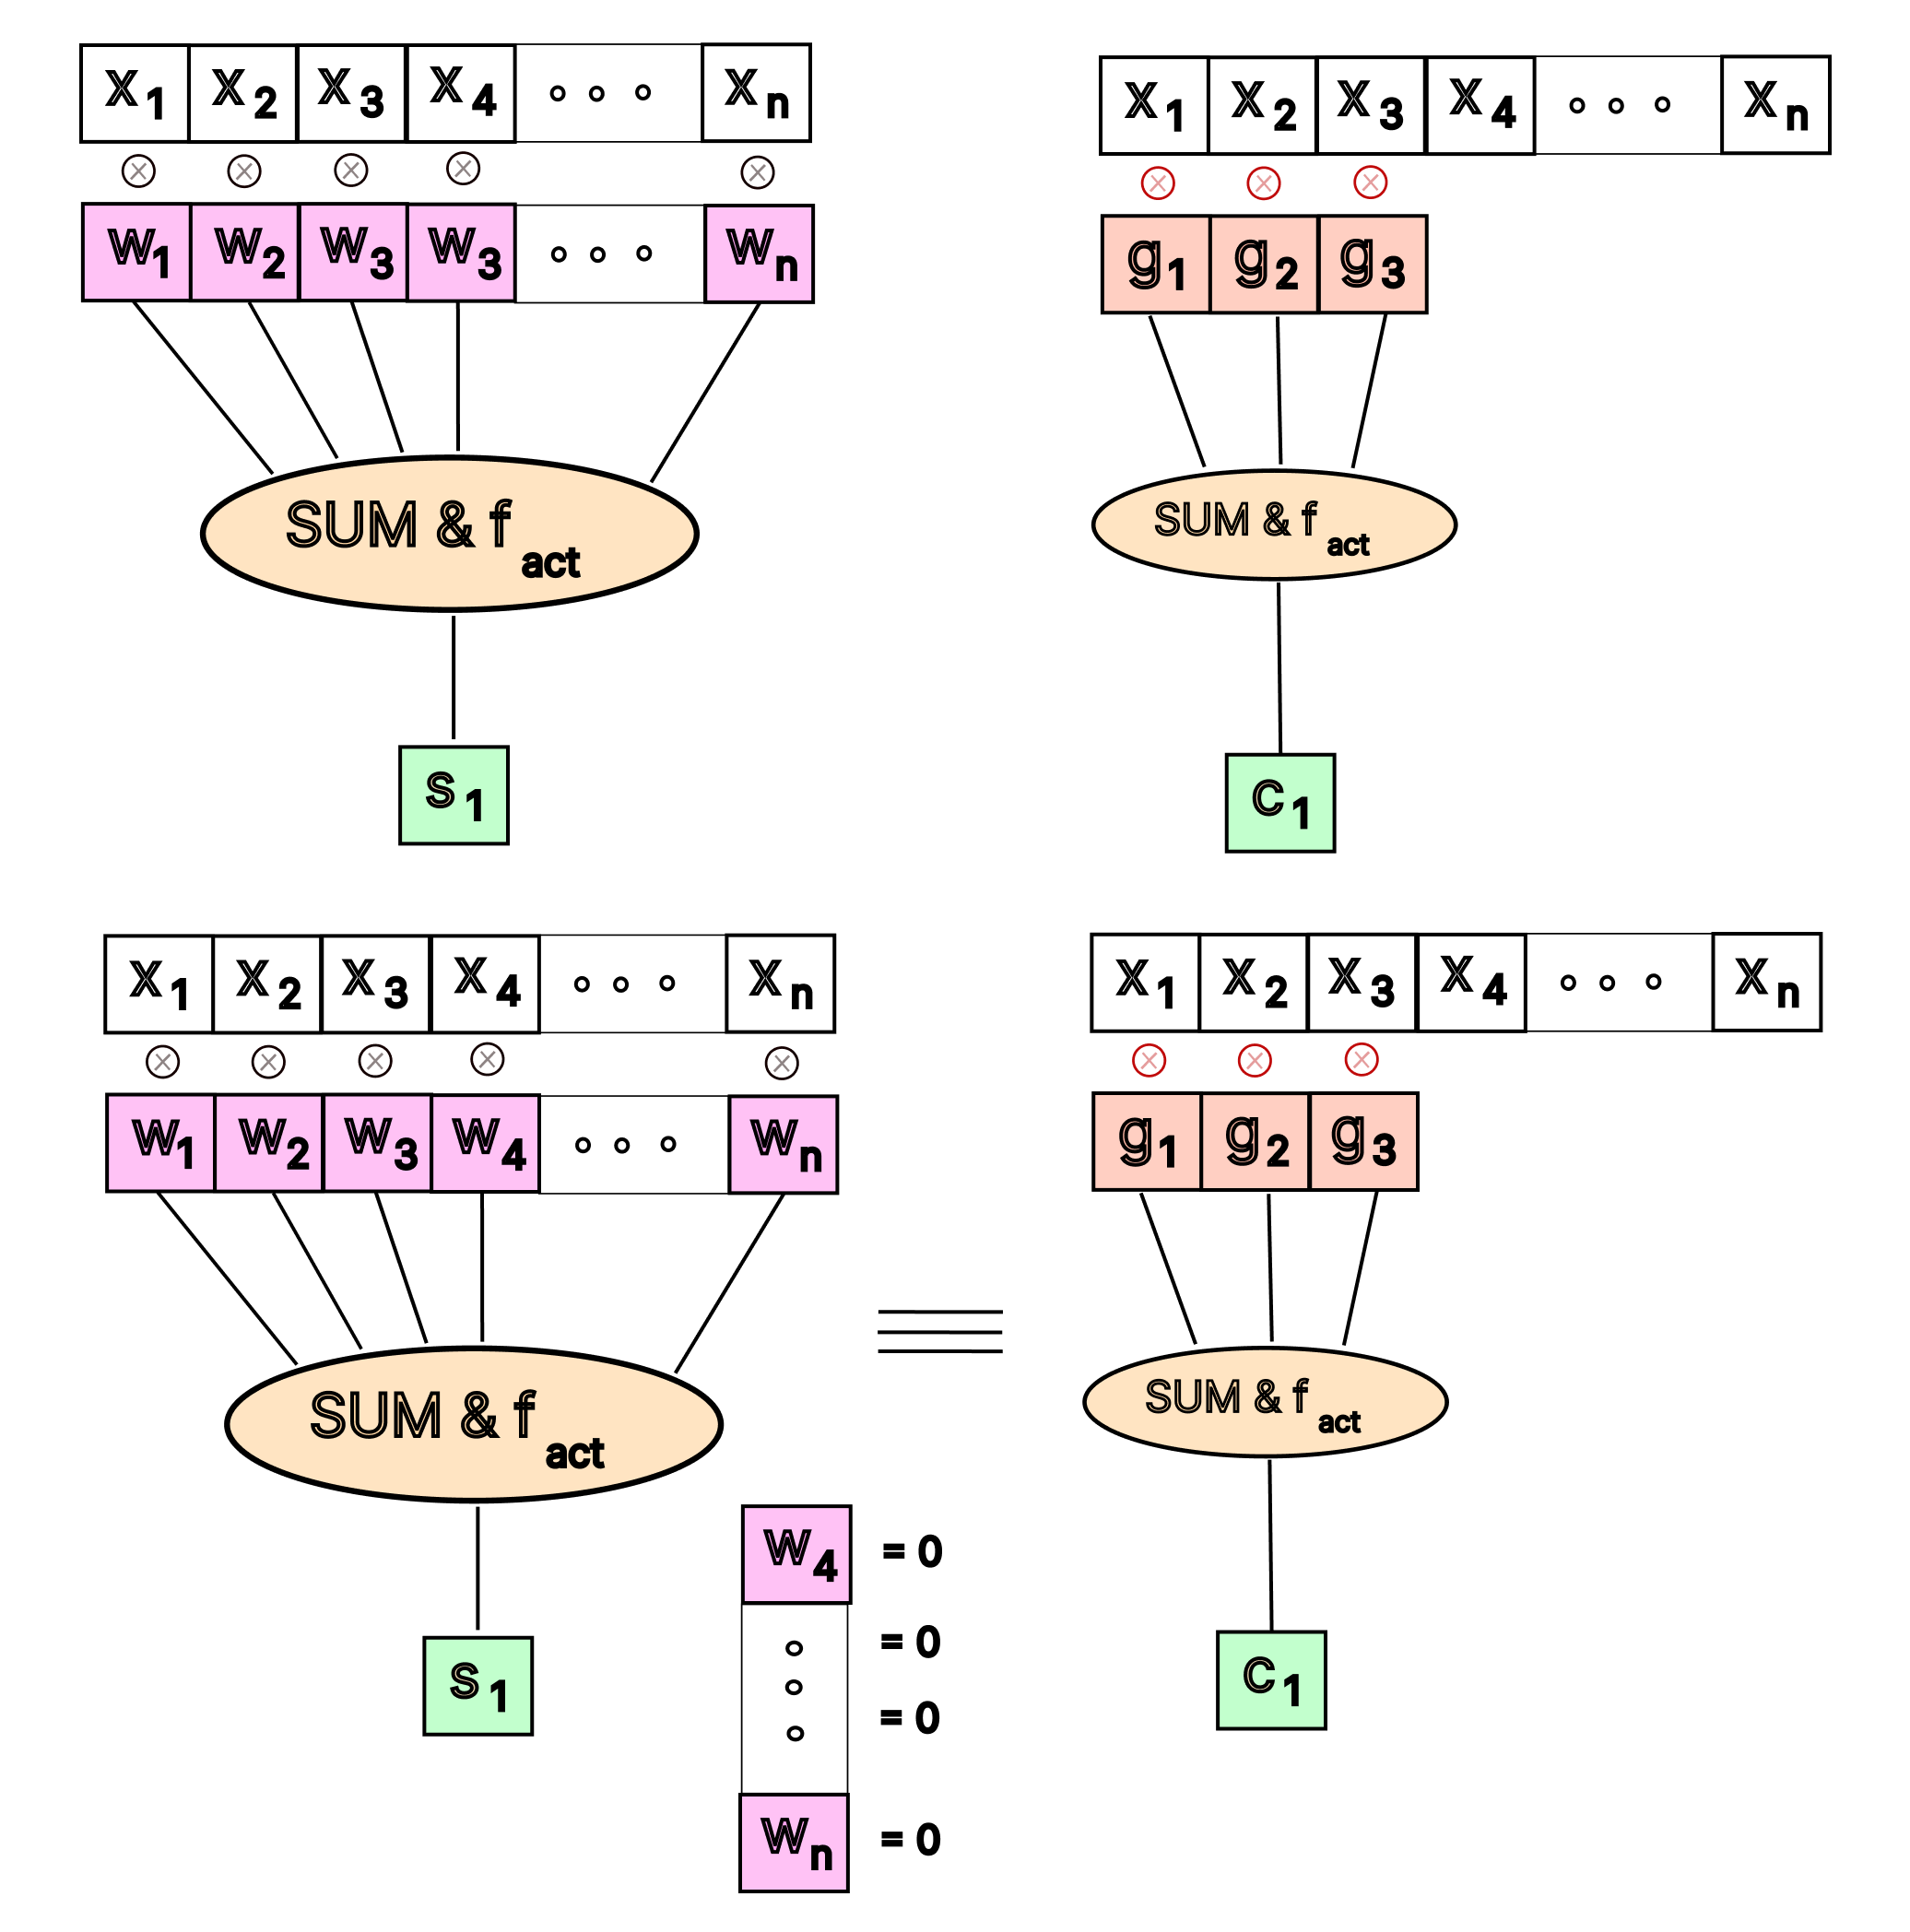
\includegraphics[width=1\linewidth]{ConvolucioENeurona.png}
    \caption{Equivalencia entre unha neurona con restricións nos pesos e un paso da convolución discreta. }
    \label{fig:exp_equivalanciaconvpercp}
\end{figure}


Tomando todo o anterior e recollendo a nosa entrada como un vector $X$, e unha función $g$ que calcularemos. A nosa función $g$ son en realidade os pesos $w_i$, bastando impoñer restricións sobre as neuronas convencionais. Por detallar a situación podemos escribir todos os pesos da capa a través dunha unha matriz $\mathbb{W}$ (Matriz \ref{mat_pesos}) onde o primeiro índice $j \in {0,...,k}$ indica a neurona e o segundo índice $i \in {0,...n}$ indica a entrada da capa á que afecta. Coa mesma idea, podemos impoñer restricións sobre a matriz de pesos para obter a convolución (Matriz \ref{mat_pesosrestriccions}), onde é importante notar que $w_{j,i} = w_{j-1, i-1}$. Deste xeito, vemos o desprazamento do \textbf{kernel}. 

\begin{figure}[h]
    \begin{equation}
    \begin{bmatrix}
    w_{11} & w_{12} & \ldots & w_{1n} \\
    w_{21} & w_{22} & \ldots & w_{2n} \\
    \vdots & \vdots & \ddots & \vdots \\
    w_{k1} & w_{k2} & \ldots & w_{kn}
    \end{bmatrix} = \mathbb{W}
    \end{equation}
    \caption{Matriz de pesos xeral dunha capa.}
    \label{mat_pesos}
\end{figure}


\begin{figure}[h]
    \centering
    \begin{equation}
    \begin{bmatrix}
    w_{11} & w_{12} & w_{13} & 0 &\ldots & 0 \\
    0 & w_{22} & w_{23} & w_{24} &\ldots & 0 \\
    \vdots & \vdots & \vdots & \vdots & \ddots & \vdots\\
    0 & 0 & 0 & w_{n(n-1)} & w_{n(n-1)} & w_{nn}
    \end{bmatrix} 
    = 
    \mathbb{G}
    =
    \begin{bmatrix}
    g_{1} & g_{2} & g_{3} & 0 &\ldots & 0 \\
    0 & g_{1} & g_{2} & g_{3} &\ldots & 0 \\
    \vdots & \vdots & \vdots & \vdots & \ddots & \vdots\\
    0 & 0 & 0 & g_{1} & g_{2} & g_{3}
    \end{bmatrix} 
    \end{equation}
    \caption{Matriz de pesos equivalente a aplicar convolución discreta.}
    \label{mat_pesosrestriccions}
\end{figure}



\textit{\textbf{Nota 1:} Estamos ignorando o nesgo (bias) de cada neurona xa que non ten valor para o noso caso. Con todo, destacar que tamén pode ser empregado na convolución. De calquera xeito, pode ser visto con un peso $w_b$ que se multiplica por un $x_b := 1$.}

A gran vantaxe desta estratexia é que reducimos enormemente o número de parámetros que precisamos adestrar e almacenar en cada capa a vez que entendemos mellor que esta aprendendo o noso modelo. 

Destacar que ao falar dunha imaxe, xa non falamos dunha convolución nunha soa dimensión, pola contra temos dous dimensións. É habitual, en moitos eidos, falar de imaxe como un sinal 2D. Así podemos ver a idea de convolución na Figura \ref{fig:imaxe_conv}.

\begin{figure}[h]
    \centering
    
\begin{tikzpicture}[
    2d-arr/.style={matrix of nodes, row sep=-\pgflinewidth, column sep=-\pgflinewidth, nodes={draw}}
  ]

  \matrix (mtr) [2d-arr] {
  0 & 1 & 1 & |[fill=orange!30]| 1 & |[fill=orange!30]| 0 & |[fill=orange!30]| 0 & 0\\
  0 & 0 & 1 & |[fill=orange!30]| 1 & |[fill=orange!30]| 1 & |[fill=orange!30]| 0 & 0\\
  0 & 0 & 0 & |[fill=orange!30]| 1 & |[fill=orange!30]| 1 & |[fill=orange!30]| 1 & 0\\
  0 & 0 & 0 & 1 & 1 & 0 & 0\\
  0 & 0 & 1 & 1 & 0 & 0 & 0\\
  0 & 1 & 1 & 0 & 0 & 0 & 0\\
  1 & 1 & 0 & 0 & 0 & 0 & 0\\
  };

  \node[below=of mtr-5-4] {$\mathbf I$};

  \node[right=0.2em of mtr] (str) {$*$};

  \matrix (K) [2d-arr, right=0.2em of str, nodes={draw, fill=teal!30}] {
    1 & 0 & 1 \\
    0 & 1 & 0 \\
    1 & 0 & 1 \\
  };
  \node[below=of K-3-2] {$\mathbf K$};

  \node[right=0.2em of K] (eq) {$=$};

  \matrix (ret) [2d-arr, right=0.2em of eq] {
  1 & 4 & 3 & |[fill=blue!80!black!30]| 4 & 1\\
  1 & 2 & 4 & 3 & 3\\
  1 & 2 & 3 & 4 & 1\\
  1 & 3 & 3 & 1 & 1\\
  3 & 3 & 1 & 1 & 0\\
  };
  \node[below=of ret-4-3] {$\mathbf{I * K}$};

  \draw[dashed, teal] (mtr-1-6.north east) -- (K-1-1.north west);
  \draw[dashed, teal] (mtr-3-6.south east) -- (K-3-1.south west);

  \draw[dashed, blue!80!black] (K-1-3.north east) -- (ret-1-4.north west);
  \draw[dashed, blue!80!black] (K-3-3.south east) -- (ret-1-4.south west);

  \foreach \i in {1,2,3} {
      \foreach \j in {4,5,6} {
          \node[font=\tiny, scale=0.6, shift={(-1.2ex,-2ex)}] at (mtr-\i-\j) {$\times \pgfmathparse{int(mod(\i+\j,2))}\pgfmathresult$};
        }
    }

\end{tikzpicture}
    \caption{Exemplo de conolución sobre unha imaxe.}
    \label{fig:imaxe_conv}
\end{figure}


\end{document}
